% This is LLNCS.DEM the demonstration file of
% the LaTeX macro package from Springer-Verlag
% for Lecture Notes in Computer Science,
% version 2.4 for LaTeX2e as of 16. April 2010
%

\documentclass{llncs}
\usepackage{amsmath}
\usepackage{german}
\usepackage{graphicx}
\usepackage{wrapfig}
\usepackage[utf8]{inputenc}
\usepackage[T1]{fontenc}
\usepackage{makeidx}  % allows for indexgeneration
\usepackage{caption}
\usepackage{tikz}
\usetikzlibrary{shapes,arrows}
%%%<
\usepackage{verbatim}
%\usepackage[active,tightpage]{preview}
%\PreviewEnvironment{tikzpicture}
%\setlength\PreviewBorder{5pt}%
%
\begin{document}
%
\mainmatter              % start of the contributions
%
\title{Übungsaufgabe 0.2: Rezept für Welfencreme}
%
\titlerunning{Formale Simulation und Verifikation verteilter Algorithmen SS17}  % abbreviated title (for running head)
%                                     also used for the TOC unless
%                                     \toctitle is used
%
\author{Jan Scholz, Lukas Kozlowski}
%
\authorrunning{Jan Scholz, Lukas Kozlowski} % abbreviated author list (for running head)
%
%%%% list of authors for the TOC (use if author list has to be modified)
\tocauthor{Jan Scholz, Lukas Kozlowski}
%
\institute{Hochschule für angewandte Wissenschaften Hamburg,\\
\email{jan.scholz2@haw-hamburg.de}\\
\email{lukas.kozlowski@haw-hamburg.de}}

\maketitle              % typeset the title of the contribution

%\begin{abstract}

%\end{abstract}
%


\section*{Aufgabe 1} % (fold)
\label{sec:aufgabe_1}
\begin{figure}[ht]
  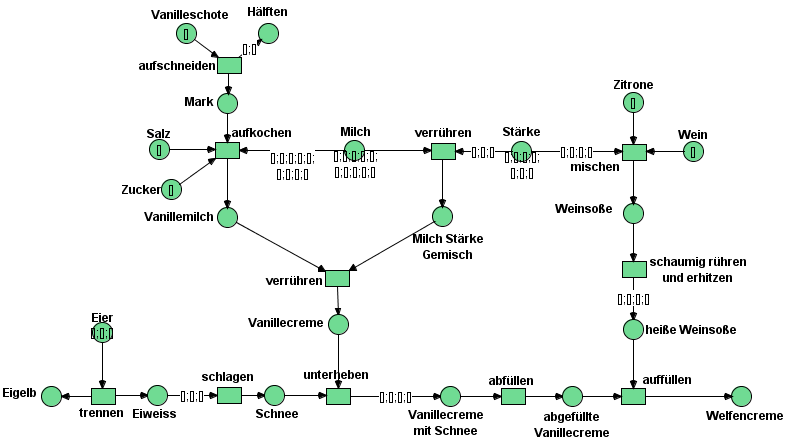
\includegraphics[width=1.3\textwidth]{pics/sim.png}
  \caption{Das auf Basis der Rezeptur erstellte Petrinetz}
  \label{pic:petrinetz}
\end{figure}
% section aufgabe_1 (end) %Jan
\section*{Aufgabe 2} % (fold)
\label{sec:aufgabe_2}
Die Initalmarkierungen $m_0$ sind wie folgt:
\begin{equation*}
	m_0 = Vanilleschote + Salz + Milch^9 + St"arke^7 + Zitronensaft + Wein + Zucker + Ei^3 
\end{equation*}

Die Aufschlüsselunge der dazugehörigen Mengen je Platz und Markierung ist wie folgt:
\begin{align*}
	Milch &= 0,05l\\
    Zucker &= 40g\\
    Salz &= 1\ Spur\\
    Vanillestange &= 1\ St"uck\\
    Speisest"arke &= 10g\\
    Ei &= 1\ St"uck\\
    Wein &= \frac{1}{4}\ l\\
    Zirtronesaft &= 1\ El.\\
\end{align*}

Alle nicht genannten Plätze haben entweder unbestimmte Mengen pro Markierung oder sind mit 1 Stück definiert.

% section aufgabe_2 (end) %Jan
\section*{Aufgabe 3} % (fold)
\label{sec:aufgabe_3}

% section aufgabe_3 (end) %Lukas 
\section*{Aufgabe 4} % (fold)
\label{sec:aufgabe_4}

% section aufgabe_4 (end) %Lukas
\section*{Aufgabe 5} % (fold)
\label{sec:aufgabe_5}

% section aufgabe_5 (end) %Lukas
\section*{Aufgabe 6} % (fold)
\label{sec:aufgabe_6}

\begin{center}
  
\tikzstyle{block} = [rectangle, draw, fill=blue!20, 
    text width=5em, text centered, rounded corners, minimum height=4em]
\tikzstyle{line} = [draw, -latex']
\tikzstyle{cloud} = [draw, ellipse,fill=red!20, node distance=3cm,
    minimum height=2em]
    
\begin{tikzpicture}[node distance = 2cm, auto]
    % Place nodes
    \node [cloud] (k1) {Koch 1};
    \node [block, below of=k1] (aufschneiden) {aufschneiden};
    \node [block, below of=aufschneiden] (aufkochen) {aufkochen};
    \node at (0,-8) [block] (unterheben) {unterheben};
    \node at (0,-10) [block] (ab1) {abfüllen};
    \node at (0,-12) [block] (auf1) {auffüllen};



    \node [cloud,right of=k1] (k2) {Koch 2};
    \node [block, below of=k2] (verrühren) {verrühren};
    \node at (3,-6) [block] (einrühren) {einrühren};
    \node at (3,-10) [block] (ab2) {abfüllen};
    \node at (3,-12) [block] (auf2) {auffüllen};


    \node [cloud,right of=k2] (k3) {Koch 3};
    \node [block, below of=k3] (mischen) {mischen};
    \node [block, below of=mischen] (schaumig) {schaumig rühren und erhitzen};
    \node at (6,-10) [block] (ab3) {abfüllen};
    \node at (6,-12) [block] (auf3) {auffüllen};
    

    \node [cloud,right of=k3] (k4) {Koch 4};
    \node [block, below of=k4] (t1) {trennen};
    \node [block, below of=t1] (t2) {trennen};
    \node [block, below of=t2] (t3) {trennen};
    \node [block, below of=t3] (schlagen) {schlagen};
    \node at (9,-10) [block] (ab4) {abfüllen};
    \node at (9,-12) [block] (auf4) {auffüllen};

    
    %\node [block, left of=evaluate, node distance=3cm] (update) {update model};
    %\node [block, below of=decide, node distance=3cm] (stop) {stop};
    % Draw edges
    \path [line] (k1) -- (aufschneiden);
    \path [line] (aufschneiden) -- (aufkochen);
    \path [line] (aufkochen) -- (unterheben);
    \path [line] (unterheben) -- (ab1);
    \path [line] (ab1) -- (auf1);

    \path [line] (k2) -- (verrühren);
    \path [line] (verrühren) -- (einrühren);
    \path [line] (einrühren) -- (ab2);
    \path [line] (ab2) -- (auf2);


    \path [line] (k3) -- (mischen);
    \path [line] (mischen) -- (schaumig);
    \path [line] (schaumig) -- (ab3);
    \path [line] (ab3) -- (auf3);

    \path [line] (k4) -- (t1);
    \path [line] (t1) -- (t2);
    \path [line] (t2) -- (t3);
    \path [line] (t3) -- (schlagen);
    \path [line] (schlagen) -- (ab4);
    \path [line] (ab4) -- (auf4);
    %\path [line] (evaluate) -- (decide);
    %\path [line] (decide) -| node [near start] {yes} (update);
    %\path [line] (update) |- (identify);
    %\path [line] (decide) -- node {no}(stop);
    %\path [line,dashed] (expert) -- (init);
    %\path [line,dashed] (system) -- (init);
    %\path [line,dashed] (system) |- (evaluate);
\end{tikzpicture}
\captionof{figure}{Flowchart für die Transitionen von 4 Köchen, Transitionen auf gleicher Höhe können parallel geschehen.}
\sffamily
  \footnotesize
% section aufgabe_6 (end)
\end{center} %Jan

%\nocite{*}
%\bibliographystyle{IEEEbib}
%\bibliography{biblio}
%\clearpage
%\addtocmark[2]{Author Index} % additional numbered TOC entry
\renewcommand{\indexname}{Author Index}
\printindex
\end{document}
